\section{Pianificazione}
Lo sviluppo del progetto è diviso nelle seguenti fasi consecutive.
\begin{enumerate}
	\item Analisi dei requisiti;
	\item Progettazione architetturale;
	\item Progettazione di dettaglio e codifica;
	\item Validazione e collaudo.
\end{enumerate}
Ogni fase è costituita da periodi, nei quali sono raggruppate le attività da svolgere.
I periodi e le attività delle prime due fasi sono individuati con una maggiore precisione rispetto a quelli successivi. Questo è dovuto alla difficoltà nel prevedere le modalità e i tempi richiesti dalle fasi più remote del progetto.
Nei \glock{diagrammi di Gantt} le barre verdi indicano attività di verifica.

Oltre alle attività riportate di seguito, verranno svolte le attività accessorie consistenti nelle riunioni interne ed esterne e produzione dei relativi verbali. Queste attività coinvolgono tutti i componenti e tutti i ruoli attivi nella fase. 

\subsection{Analisi dei requisiti (dal 2020-10-22 al 2021-01-17)}

\subsubsection{Ruoli attivi}
\begin{itemize}
	\item Responsabile;
	\item Amministratore;
	\item Analista;
	\item Verificatore.
\end{itemize}

\subsubsection{Periodi e attività}

\paragraph{Primo periodo (dal 2020-10-22 al 2020-11-09)}
Questo periodo comincia con la costituzione del gruppo di progetto. Serve dunque a porre le basi per una comunicazione e collaborazione efficace ed efficiente. Vi si svolgono inoltre attività di ricerca superficiale sui capitolati.

\begin{itemize}
	\item Configurazione degli strumenti collaborativi basilari: comprende la scelta e la configurazione dei mezzi per la comunicazione e il lavoro collaborativo;
	\item Analisi superficiale dei capitolati.
	
\end{itemize}

\paragraph{Secondo Periodo (dal 2020-11-10 al 2020-12-13)}
Gli obiettivi raggiunti in questo periodo sono il consolidamento degli strumenti di collaborazione e l'approfondimento dei capitolati.
\begin{itemize}
	\item Configurazione del \glock{repository}: questa attività comprende la creazione di un repository per la condivisione e il versionamento dei prodotti, ma anche la sua configurazione per la verifica automatica della loro validità;
	\item Raccolta di informazioni dai seminari: stesura di appunti sui seminari, da poter facilmente consultare quando necessario;
	\item Studio dei progetti degli anni passati: questa attività ha il fine di individuare gli errori più comuni e le tecniche da prendere come esempio;
	\item Bozza dello studio di fattibilità;
	\item Bozza delle norme di progetto.
\end{itemize}

\paragraph{Terzo Periodo (dal 2020-12-14 al 2020-01-08)}
Questo periodo segue la scelta del capitolato da affrontare. È dedicato alla sua analisi approfondita e alla stesura della documentazione. 
\begin{itemize}
	\item Stesura delle norme di progetto;
	\item Stesura dello studio di fattibilità;
	\item Stesura del piano di progetto;
	\item Analisi dei requisiti e stesura dell'omonimo documento;
	\item Stesura del piano di qualifica;
	\item Stesura del glossario;
	\item Stesura della lettera di presentazione;
	\item Aggiornamento consuntivo;
	\item Verifica della documentazione.
\end{itemize}

\paragraph{Quarto Periodo (dal 2020-01-09 al 2020-01-17)}
Questo periodo è l'ultimo della fase di analisi dei requisiti. Si concentra quindi sulla preparazione dell'esposizione dei prodotti dei tre periodi precedenti.
\begin{itemize}
	\item Preparazione dell'esposizione;
	\item Verifica dell'esposizione.
\end{itemize}


\begin{landscape}
	\begin{figure}[H]
		\centering
		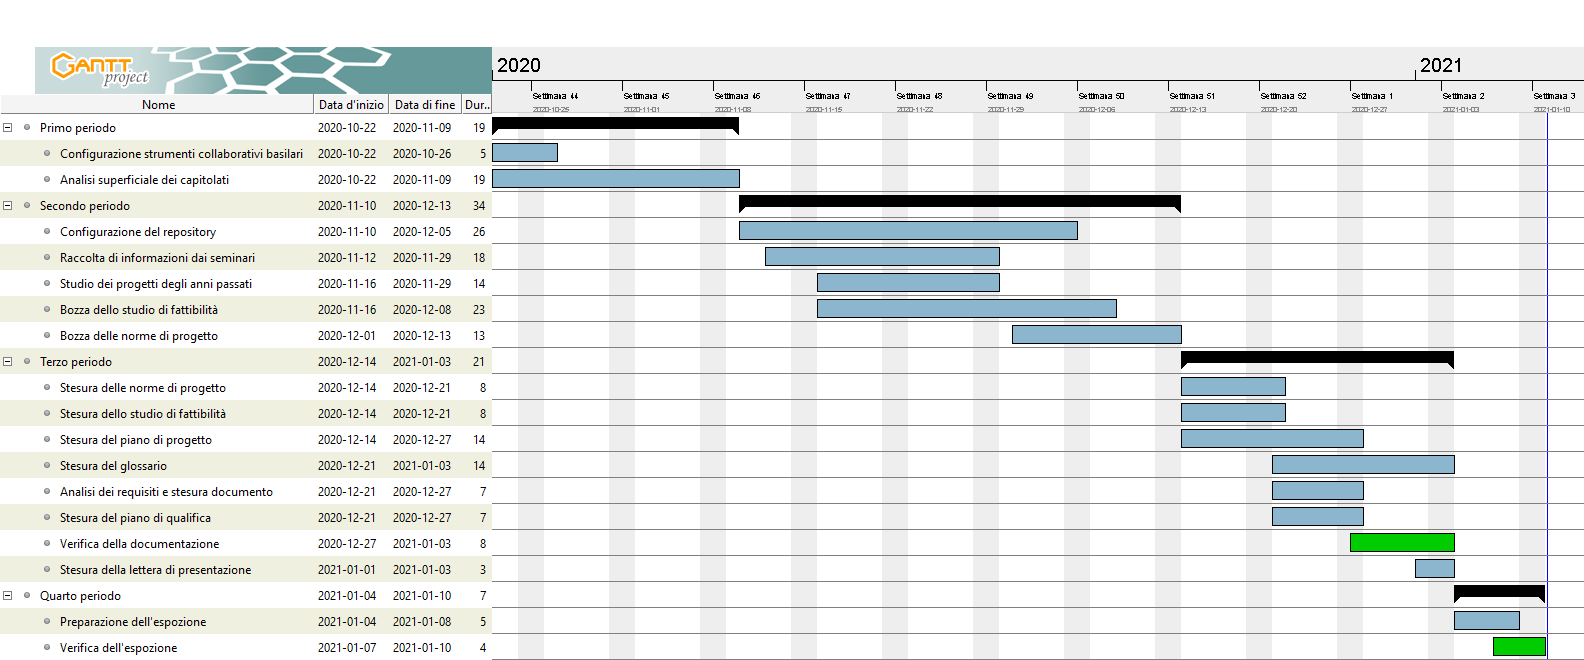
\includegraphics[width=\linewidth]{res/images/ganttFase1.png}
		\caption*{\textbf{Figura 1}{: Grafico di Gantt della fase di analisi dei requisiti}}
		\label{fig:Gantt Analisi dei requisiti}
	\end{figure}
\end{landscape}

\subsection{Progettazione architetturale (dal 2021-01-18 al 2021-03-07)}

\subsubsection{Ruoli attivi}
\begin{itemize}
	\item Responsabile;
	\item Amministratore;
	\item Analista;
	\item Progettista;
	\item Verificatore.
\end{itemize}

\subsubsection{Periodi e attività}

\paragraph{Primo Periodo (dal 2021-01-18 al 2021-01-20)}
\begin{itemize}
	\item Aggiornamento Norme di progetto;
	\item Aggiornamento Piano di qualifica;
	\item Aggiornamento pianificazione;
	\item Verifica documentazione.
\end{itemize}

\paragraph{Secondo Periodo (dal 2021-01-21 al 2021-02-19)}
\begin{itemize}
	\item Aggiornamento requisiti;
	\item Ricerca: si esegue attività di ricerca sulle architetture più adatte al prodotto da sviluppare e alla soddisfazione dei requisiti richiesti;
	\item Progettazione: si costruisce un modello del prodotto che si vuole ottenere, definendone l'architettura;
	\item Verifica.
\end{itemize}

\paragraph{Terzo Periodo (dal 2021-02-20 al 2021-02-27)}
\begin{itemize}
	\item Progettazione \glock{Proof of concept};
	\item Codifica Proof of concept;
	\item Redazione della  \glock{Technology baseline};
	\item Verifica Proof of Concept e Technology baseline.
\end{itemize}

\paragraph{Quarto Periodo (dal 2021-02-28 al 2021-03-07)}
\begin{itemize}
	\item Stesura Lettera di presentazione;
	\item Aggiornamento consuntivo;
	\item Verifica documentazione;
	\item Preparazione presentazione;
	\item Verifica della presentazione.
\end{itemize}

\begin{landscape}
	\begin{figure}[H]
		\centering
		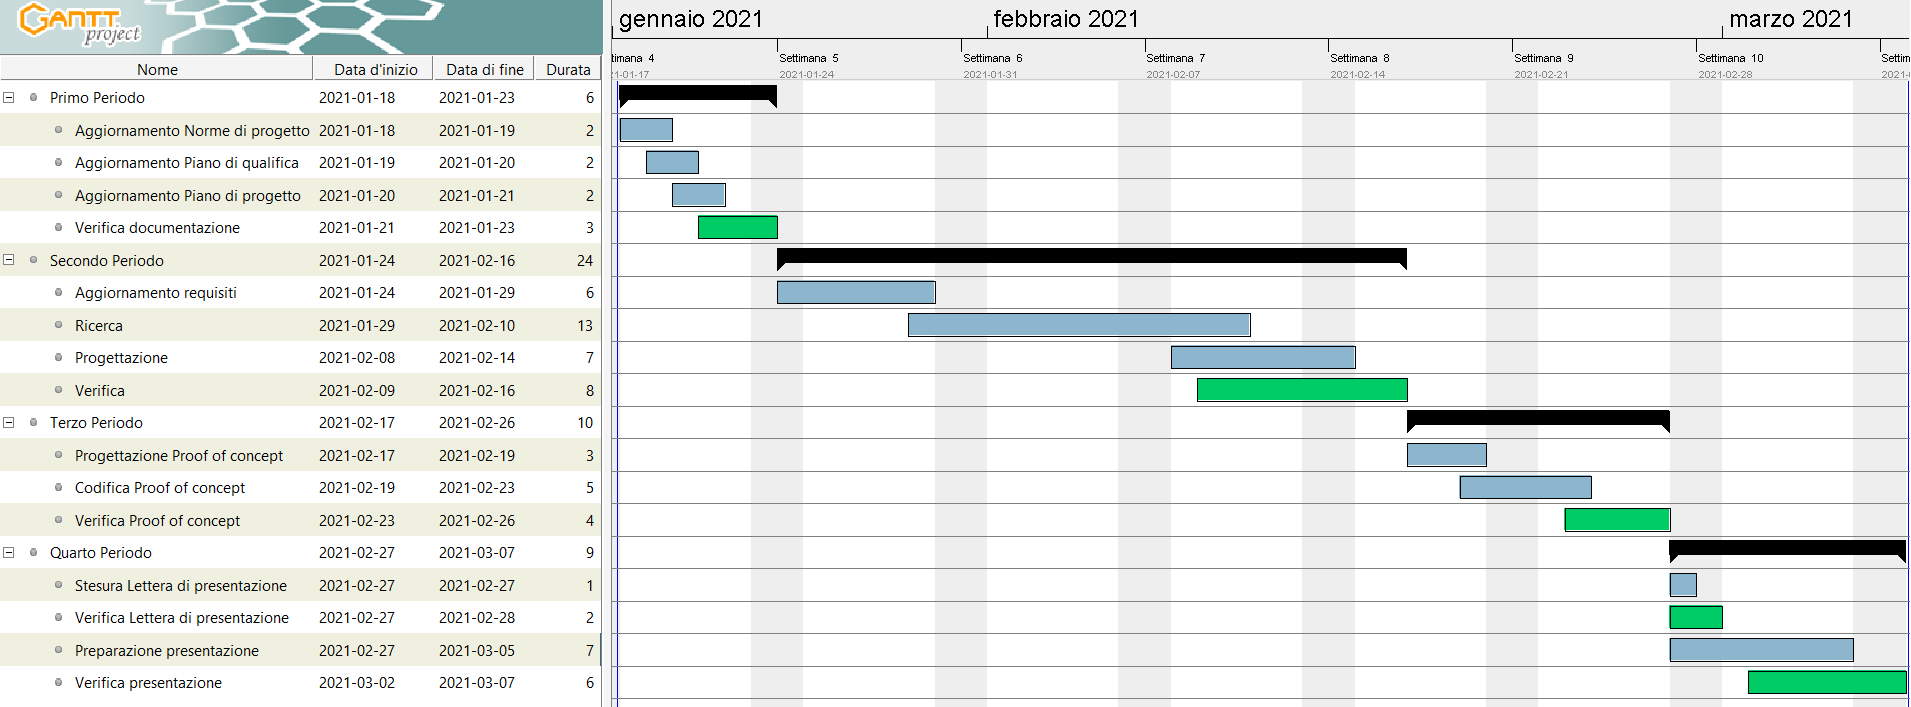
\includegraphics[width=\linewidth]{res/images/ganttFase2.png}
		\caption*{\textbf{Figura 2}{: Grafico di Gantt della fase di Progettazione architetturale}}
		\label{fig:Gantt Analisi dei requisiti}
	\end{figure}
\end{landscape}

\subsection{Progettazione di dettaglio e codifica (dal 2021-03-08 al 2021-04-08)}

\subsubsection{Ruoli attivi}
\begin{itemize}
	\item Responsabile;
	\item Amministratore;
	\item Analista;
	\item Progettista;
	\item Programmatore;
	\item Verificatore.
\end{itemize}

\subsubsection{Periodi e attività}

\paragraph{Primo Periodo (dal 2021-03-08 al 2021-03-09)}
\begin{itemize}
	\item Aggiornamento Norme di progetto;
	\item Aggiornamento Piano di qualifica;
	\item Aggiornamento pianificazione;
	\item Verifica documentazione.
\end{itemize}

\paragraph{Secondo Periodo (dal 2021-03-10 al 2021-03-12)}
\begin{itemize}
	\item Stesura  \glock{Product baseline};
	\item Verifica Product baseline.
\end{itemize}

\paragraph{Terzo Periodo - Incremento I (dal 2021-03-13 al 2021-03-19)}
\begin{itemize}
	\item Codifica della struttura delle componenti: sono implementate quelle funzionalità del web server e dell'applicazione che non necessitano di un'interazione con le altre componenti del sistema. In questo incremento l'unico requisito funzionale che viene corrisposto pienamente è il R2F1. Tuttavia il I incremento pone le basi per il lavoro degli incrementi successivi;
	\item Verifica.
\end{itemize}

\paragraph{Quarto Periodo - Incremento II (dal 2021-03-20 al 2021-03-24)}
\begin{itemize}
	\item  Codifica delle interazioni tra le componenti interne: sono implementate le interazioni tra web server e applicazione per telefono. I requisiti funzionali soddisfatti in questo periodo sono: R1F2, R1F2.1, R1F2.2, R1F3, R1F4, R1F4.1, R1F4.2, R1F4.3, R1F4.4, R1F4.5, R1F4.6, R1F4.8, R1F4.10, R1F4.11, R1F4.12, R1F4.13, R1F4.14, R1F4.16, R1F4.18, R1F4.20, R1F4.21, R1F5, R1F5.1, R1F5.2, R1F5.3, R1F5.4, R1F5.5, R1F6, R1F6.1, R1F6.1.1, R2F6.1.2, R1F6.2, R1F6.2.1, R1F6.3, R2F6.3.1, R2F7, R2F7.1, R2F7.1.1, R1F8, R1F9, R1F9.1, R1F10, R1F10.1, R1F10.2, R1F11, R1F11.1, R1F11.2, R1F11.3, R1F11.4, R1F12, R1F12.1, R1F12.2, R1F13, R1F13.1, R1F13.2, R1F13.3;
	\item Verifica.
\end{itemize}

\paragraph{Quinto Periodo - Incremento III (dal 2021-03-25 al 2021-03-29)}
\begin{itemize}
	\item Codifica delle interazioni con gli attori esterni: sono implementate le interazioni tra web server e servizio \glock{Ethereum} e quelle tra applicazione per telefono e \glock{tag RFID}.
	I requisiti corrisposti in questo periodo sono: R1F4.7, R1F4.9, R1F4.15, R1F4.17, R1F4.19;
	\item Verifica.
\end{itemize}

\paragraph{Sesto Periodo - Incremento IV (dal 2021-03-30 al 2021-03-31)}
\begin{itemize}
	\item Codifica delle funzionalità secondarie non ancora implementate: questo periodo è dedicato alla soddisfazione dei requisiti opzionali non ancora affrontati;
	\item Stesura manuale utente;
	\item Stesura manuale manutentore;
	\item Verifica.
\end{itemize}

\paragraph{Settimo Periodo (dal 2021-04-01 al 2021-04-08)}
\begin{itemize}
	\item Stesura Lettera di presentazione;
	\item Aggiornamento del consuntivo;
	\item Verifica della documentazione;
	\item Preparazione della presentazione;
	\item Verifica della presentazione.
\end{itemize}

\begin{landscape}
	\begin{figure}[H]
		\centering
		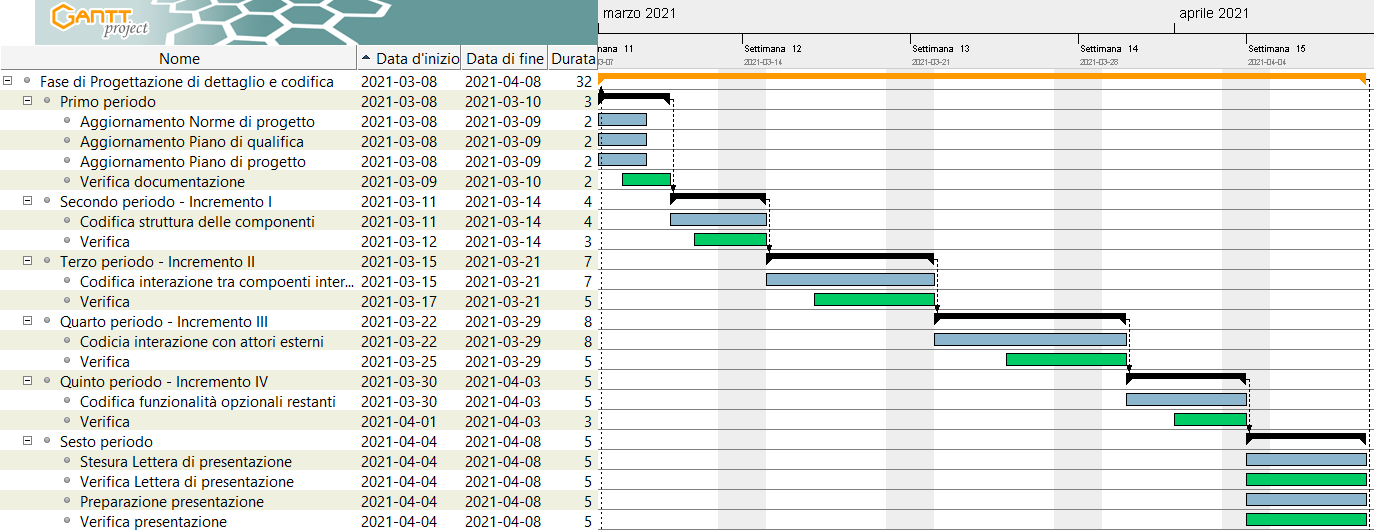
\includegraphics[width=\linewidth]{res/images/ganttFase3.png}
		\caption*{\textbf{Figura 3}{: Grafico di Gantt della fase di Progettazione architetturale}}
		\label{fig:Gantt Analisi dei requisiti}
	\end{figure}
\end{landscape}

\subsection{Validazione e collaudo (dal 2021-04-09 al 2021-05-09)}

\subsubsection{Ruoli attivi}
\begin{itemize}
	\item Responsabile;
	\item Amministratore;
	\item Progettista;
	\item Programmatore;
		\item Verificatore.
\end{itemize}

\subsubsection{Periodi e attività}

\paragraph{Primo Periodo (dal 2021-04-09 al 2021-04-13)}
\begin{itemize}
	\item Aggiornamento Norme di progetto;
	\item Aggiornamento Piano di qualifica;
	\item Aggiornamento pianificazione;
	\item Verifica documentazione.
\end{itemize}

\paragraph{Secondo Periodo (dal 2021-04-14 al 2021-04-30)}
\begin{itemize}
	\item Validazione: vengono effettuate le verifiche finali e complessive sul codice prodotto;
	\item Collaudo: viene effettuato il collaudo degli applicativi prodotti.
\end{itemize}

\paragraph{Terzo Periodo (dal 2021-05-01 al 2021-05-09)}
\begin{itemize}
	\item Stesura Lettera di presentazione;
	\item Aggiornamento del consuntivo;
	\item Verifica della documentazione;
	\item Preparazione della presentazione;
	\item Verifica della presentazione.
\end{itemize}

\begin{landscape}
	\begin{figure}[H]
		\centering
		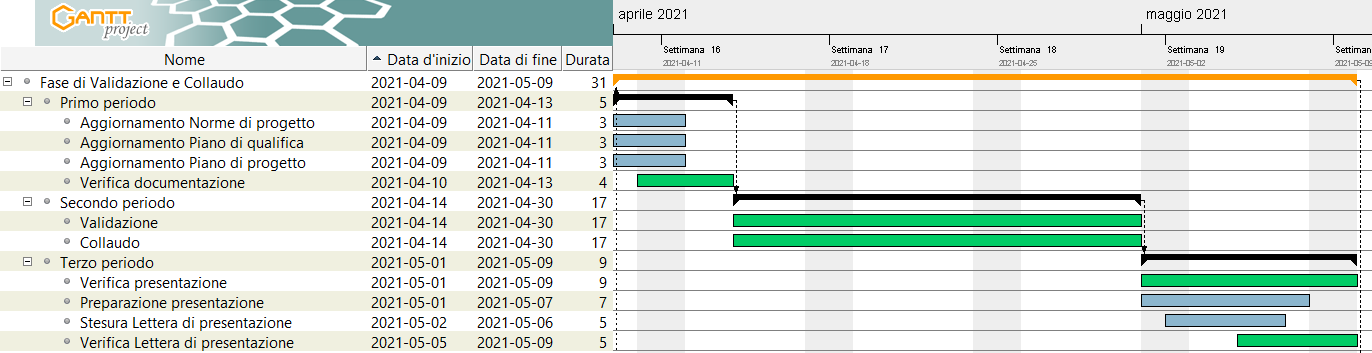
\includegraphics[width=\linewidth]{res/images/ganttFase4.png}
		\caption*{\textbf{Figura 4}{: Grafico di Gantt della fase di Validazione e collaudo}}
		\label{fig:Gantt Analisi dei requisiti}
	\end{figure}
\end{landscape}


\begin{landscape}
	\begin{figure}[H]
		\centering
		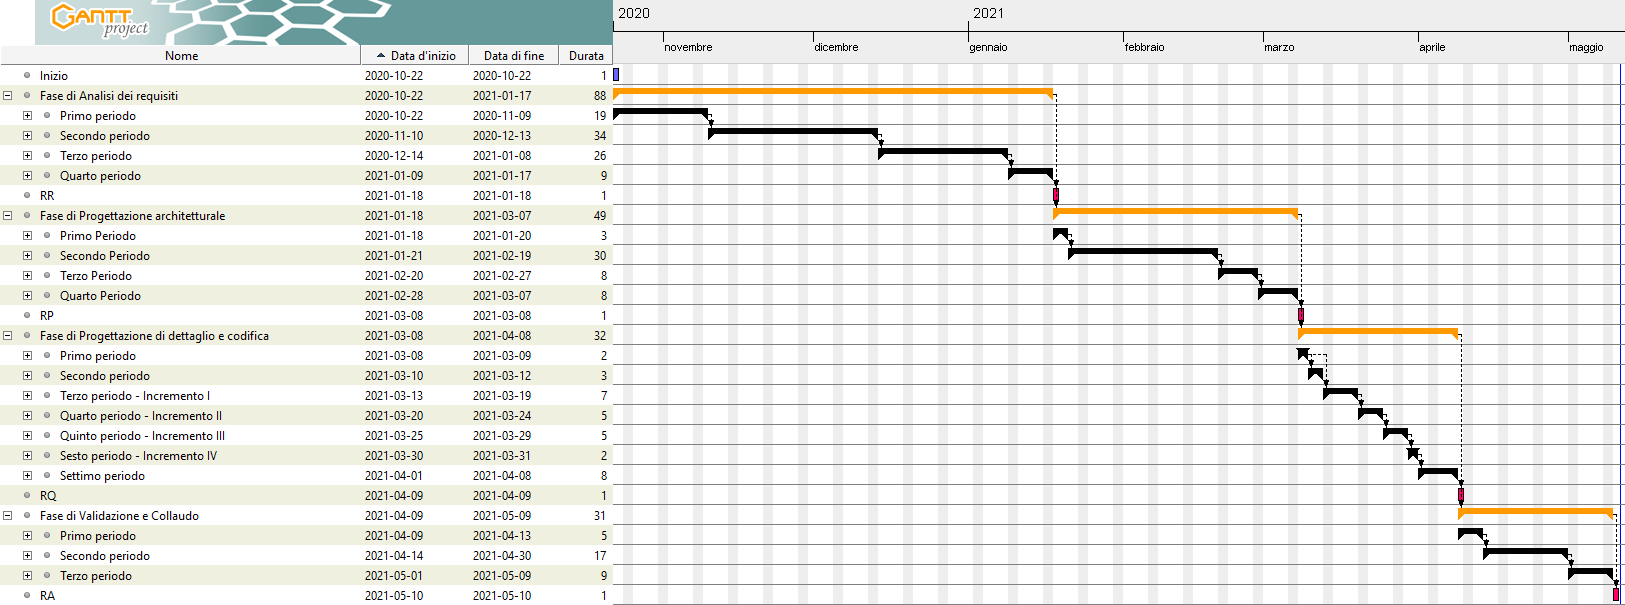
\includegraphics[width=\linewidth]{res/images/ganttTotale.png}
		\caption*{\textbf{Figura 5}: Grafico di Gantt dell'intero progetto}
		\label{fig:Gantt Analisi dei requisiti}
	\end{figure}
\end{landscape}

